\documentclass[border=10pt]{standalone}
\usepackage{pgfplots}
\pgfplotsset{compat=1.18}
\begin{document}
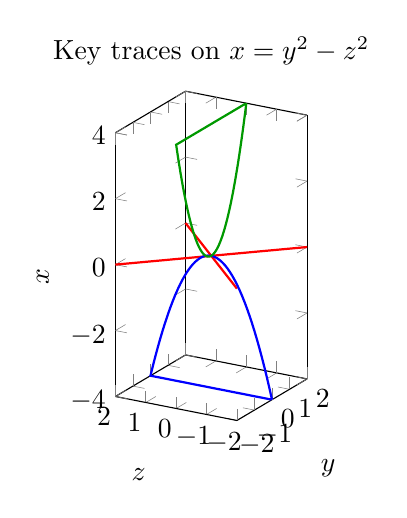
\begin{tikzpicture}
\begin{axis}[
    xlabel={$y$}, ylabel={$z$}, zlabel={$x$},
    title={Key traces on $x=y^2-z^2$},
    view={-60}{20},
    xmin=-2, xmax=2, ymin=-2, ymax=2, zmin=-4, zmax=4,
    xtick={-2,-1,0,1,2},
    ytick={-2,-1,0,1,2},
    ztick={-4,-2,0,2,4},
    unit vector ratio=1 1 1,
    legend pos=outer north east
]
% x=0 trace: y = ±z
\addplot3[red, thick, samples=20, domain=-2:2] (x,x,0);
\addplot3[red, thick, samples=20, domain=-2:2] (x,-x,0);
% y=0 trace: x = -z^2
\addplot3[blue, thick, samples=50, variable=\t, domain=-2:2] (0,\t,{-\t*\t});
% z=0 trace: x = y^2
\addplot3[green!60!black, thick, samples=50, variable=\t, domain=-2:2] (\t,0,{\t*\t});
\end{axis}
\end{tikzpicture}
\end{document}
